\documentclass[]{article}
\usepackage{graphicx}
\usepackage{subcaption}
\usepackage{amsmath}
\usepackage{amsfonts}




%opening
\title{Surrogate Modeling with Physics-Based Neural Networks}

\author{Alex Feild}

\begin{document}

\maketitle

\begin{abstract}
The purpose of surrogate modeling is to replace some target model with an approximation that mimics the target's behavior.  This is typically done to replace an explicit, explainable, but comparatively slow model with an implicit, less explainable, but much faster model.  We will define terms for this proposal as follows:  Physics-Based Machine Learning is the application of mathematical physics to machine learning.  Physics-Informed Neural Networks (PINNs) include conservation terms, in the form of partial differential equations (PDEs), as part of their loss function.  This technical section covers Physics-Based Neural Networks, with a focus on the use of applied mathematics in modeling with neural networks.  

\end{abstract}

\section{Background: Automatic Differentiation}
Automatic differentiation (autodiff) is critical to some of the techniques described in this report.  Automatic differentiation makes gradient learning methods much simpler to implement compared to analytic or numerical differentiation.  Unlike analytic differentiation, autodiff does not require the programmer to compute and provide derivatives.  Unlike numerical differentiation, autodiff gives exact results.  Autodiff is not symbolic differentiation.  Autodiff uses the chain rule:
\begin{gather}
	y = f(g(h(x)))\\
	y' = f'(g(h(x)))g'(h(x))h'(x) = \frac{df(g(h(x))}{dg(h(x))} \frac{dg(h(x))}{dh(x)} \frac{dh(x)}{dx}
\end{gather}
This is usually done with intermediate variables.  Assign:
\begin{equation}
	z_0 = x, z_1 = h(z_0), z_2 = g(z_1), z_3 = f(z_2)
\end{equation}
Then we can rewrite the rule in terms of these intermediate variables:
\begin{equation}
	\frac{dy}{dx} = \frac{dy}{dz_2} \frac{dz_2}{dz_1} \frac{dz_1}{dx} 
\end{equation}
Autodiff exploits the fact all computer calculations can be reduced to a sequence of simple operations and functions, such as add, multiple, subtract, divide, sin, cos, exp, and log.  Typically autodiff libraries record a graph of these computations.  Since these simple operations and functions have know derivatives, a graph of derivatives can also be constructed.  At the extremes there are two modes of computing the derivatives.  Forward accumulation computes the derivative of each sub-expression while holding the independent variable fixed.  And recursively substitutes the inner function with the derivative in accordance with the chain rule (while obeynig any branching in the graph).
\begin{equation}
	\frac{dy}{dx} = \prod_{l=0}^{L}\frac{dz_{0+l}}{dx}
\end{equation}
In contrast, reverse accumulation holds the dependent variable constant and recursively computes the derivative of each sub-expression (again, following any branching in the computational graph). 
\begin{equation}
	\frac{dy}{dx} = \prod_{l=0}^{L}\frac{dy}{dz_{L-l}}
\end{equation}

\begin{figure}
	\centering
	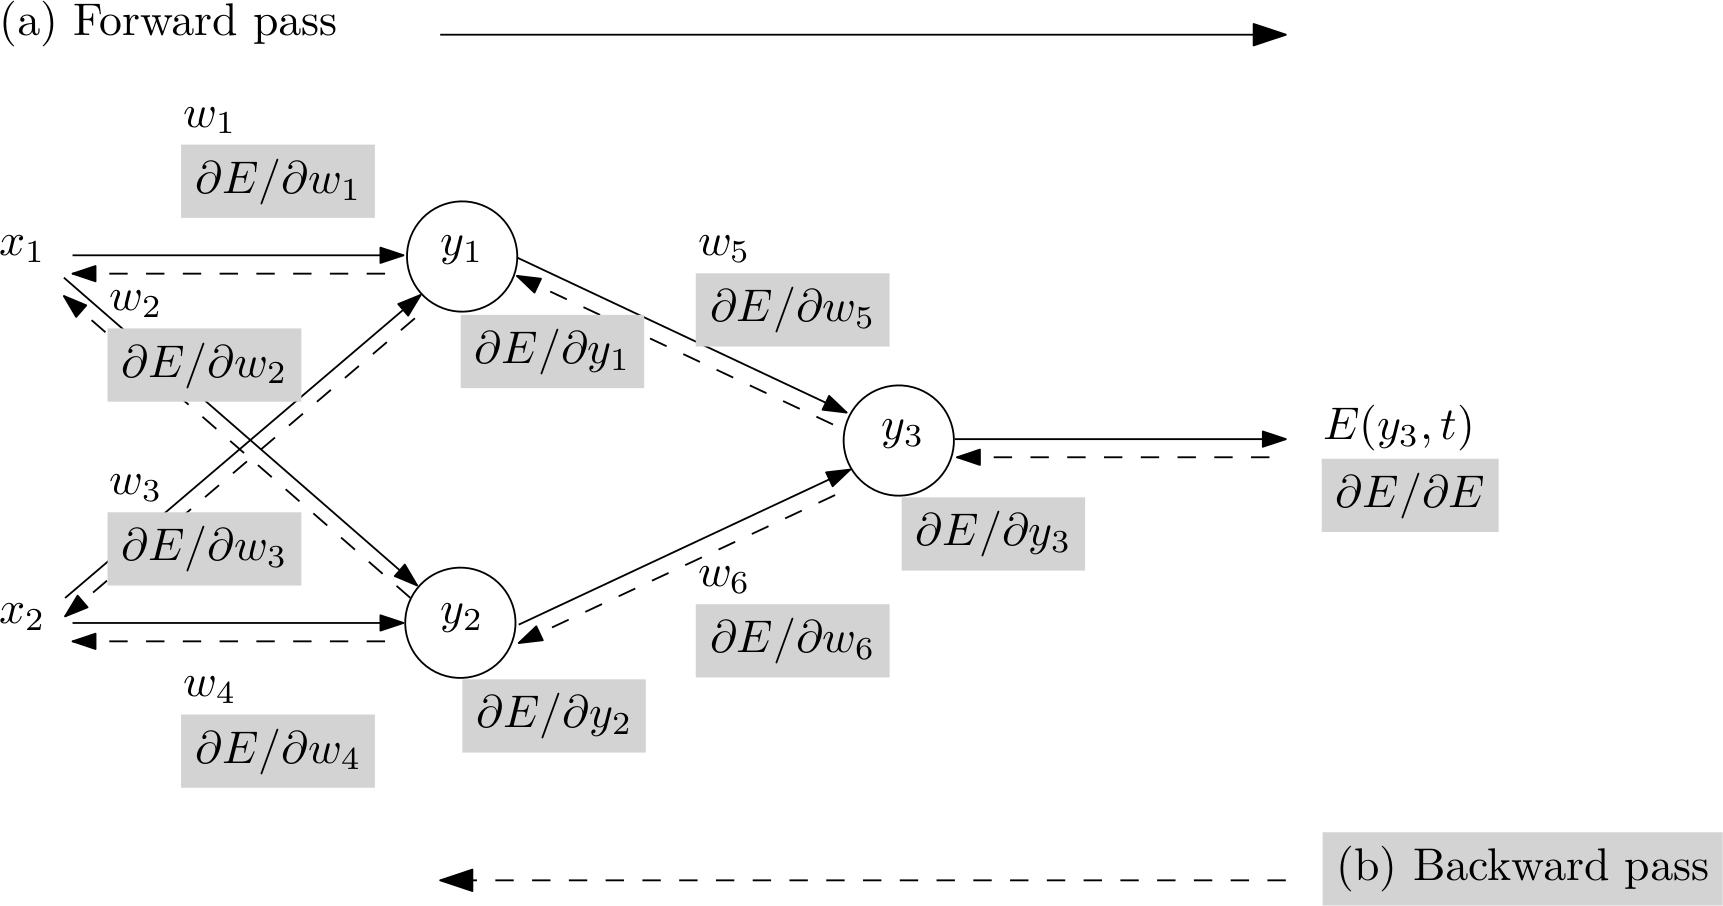
\includegraphics[width=1.0\linewidth]{images/autodiff}
	\caption[autodiff]{Autodiff graph by \cite{autodiff_survey}}
	\label{fig:autodiff}
\end{figure}

Both full forward and reverse accumulation are extreme cases.  In practice, packages like Pytorch only hold part of the graph in memory at any given moment, releasing unnecessary variables when not needed \cite{autofiff_pytorch}.

In addition to programming the known derivatives of basic operations and functions, we can use the dual numbers for automatic differentiation.  Dual numbers consist of two real numbers a and b, where b is the multiple of the abstract number $\varepsilon$, with the property $\varepsilon^2 = 0$.  The dual numbers are of the form $a + b\varepsilon$.  Using this definition we can now do some basic operations with the dual numbers:
\begin{gather}
(a + b\varepsilon) + (c + d\varepsilon) = (a + c) + (b + d)\varepsilon \\
(a + b\varepsilon) - (c + d\varepsilon) = (a - c) + (b - d)\varepsilon \\
(a + b\varepsilon) * (c + d\varepsilon) = ac + (ad + bc)\varepsilon \\
(a + b\varepsilon) / (c + d\varepsilon) = a/c + (b/c - ad/c^2)\varepsilon 
\end{gather}
The second real number in the dual number can be treated as the derivative of the first, giving $x + x'\varepsilon$.  Below are some standard function in terms of the dual numbers.
\begin{gather}
sin(x + x'\varepsilon) = sin(x) + x'cos(x)\varepsilon \\
cos(x + x'\varepsilon) = cos(x) - x'sin(x)\varepsilon \\
exp(x + x'\varepsilon) = exp(x) + x'exp(x)\varepsilon \\
log(x + x'\varepsilon) = log(x) + (x'/ x)\varepsilon \\
(x + x'\varepsilon)^k = x^k + x'kx^{k-1}\varepsilon\\
|x + x'\varepsilon| = |x| + x'signof(x)\varepsilon
\end{gather}
Dual numbers will be stored in the computer as an ordered pair $(x,x')$.  Vector gradients can be calculated by simply substituting entries with dual numbers.  Using dual numbers for automatic differentiation can be achieved via operator overloading and replacing scalar values with dual numbers.  Engineering experience shows that a computational graph for reverse mode accumulation may be more memory efficient, while forward mode accumulation with dual number may be easier to implement (via operator overloading).  

\subsection{Background: Autodiff Motivation: Backpropagation}
The purpose of backpropagation is to apply gradient descent to neural networks.  There are many modifications to the scheme in order to aviod local minima, but the basic gradient descent scheme is:
\begin{equation}
\boldsymbol{\theta}^i = \boldsymbol{\theta}^{i-1} - u^i\nabla \textbf{L}(\boldsymbol{\theta}^{i-1})
\end{equation}
Recall the basic layout of a fully connected feed forward neural network shown in Figure \ref{fig:nnfrommlbook}.  
\begin{figure}
	\centering
	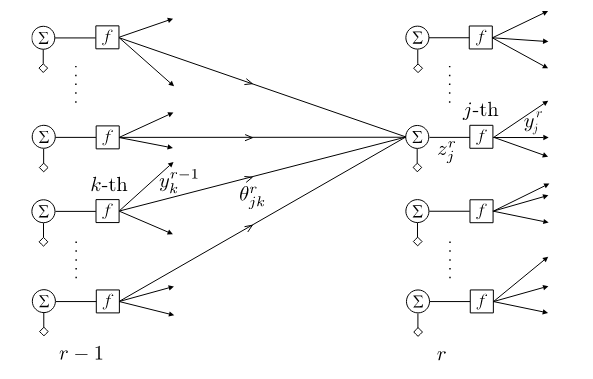
\includegraphics[width=1\linewidth]{images/nn_from_ml_book}
	\caption[ANN Labeled]{Basic neural network with layers, neurons, and weights labeled from \cite{ml_book}.}
	\label{fig:nnfrommlbook}
\end{figure}
Gradient descent for each parameter becomes:
\begin{gather}
\theta^{r,i}_{j,k} = \theta^{r,i-1}_{j,k} + \triangle\theta^{r, i -1}_{j,k} \\
\triangle\theta^{r, i -1}_{j,k} = - u^i\frac{\partial \textbf{L}}{ \theta^{r,i-1}_{j,k}}
\end{gather}
Where $i$ is the iteration or timestep, $r$ is the layer of the neuron that this parameter belongs to, $j$ is the neuron index in $r$ that the parameter $\theta$ belongs to, and $k$ is the neuron in the $r-1$ layer that this parameter connects to.  Here the convention from \cite{ml_book} where 1.0 is added to the front of $y^{r-1, i}$ so that the bias is accounted for as part of the other weights in $\theta^{r, i}_j$ is used.  Perhaps matrices will make things more clear:
\begin{equation} 
\textbf{y}^{r-1}_n = [1.0, y^{r-1}_{n,1}, ..., y_{n,K_{r-1}-1}^{r-1}]
\end{equation}
\[
{\textbf{Y}^{r-1}}^T = 
	\begin{Bmatrix}
	1 & y_{0,1}^{r-1} & ... & y_{0,K_{r-1} - 1}^{r-1}\\
	... & ... & ... & ...\\
	1 & y_{N -1,1}^{r-1} & ... & y_{N - 1,K_{r-1} - 1}^{r-1}
	\end{Bmatrix}
\]
Where $\textbf{Y}^{r-1}$ is transposed in preparation for multiplication, $K_{r-1}$ is the number of outputs coming from the $r-1$ layer, and $N$ is the number of samples in a batch.
\[
\boldsymbol{\theta}^r = 
	\begin{Bmatrix}
	\theta_{0,0}^r & ... & \theta_{J_r - 1,0}^r\\
	... & ... & ...\\
	\theta_{0,K_{r-1} - 1}^r & ... & \theta_{J_r - 1,K_{r-1} -1}^r
	\end{Bmatrix}
\]
Where $J$ is the number of neurons in this layer $r$.  Multiplying them yields:
\[
\textbf{Z}^r = {\textbf{Y}^{r-1}}^T \theta^r =
	\begin{Bmatrix}
	z_{0,0}^r & ... & z_{J_r-1,0}^r\\
	... & ... & ...\\
	z_{0,N-1}^r & ... & z_{J_r-1,N-1}^r
	\end{Bmatrix}
\]
Applying the activation function $f()$ gets $\textbf{Y}^r$.
\[
f(\textbf{Z}^r) = \textbf{Y}^r =
	\begin{Bmatrix}
	y_{0,0}^r & ... & y_{J_r-1,0}^r\\
	... & ... & ...\\
	y_{0,N-1}^r & ... & y_{J_r-1,N-1}^r
	\end{Bmatrix}
\]
If $r$ is the last layer $r = L$, the loss function will compute on all $J_L$ outputs.
\[
\textbf{Y}^L =
	\begin{Bmatrix}
	y_{0,0}^L & ... & y_{J_L-1,0}^L\\
	... & ... & ...\\
	y_{0,N-1}^L & ... & y_{J_L-1,N-1}^L
	\end{Bmatrix}
\]
\[
\textbf{L}_n(\boldsymbol{\theta}) =
	\begin{Bmatrix}
	L_0\\
	...\\
	L_{N-1}
	\end{Bmatrix}
\]
\begin{equation}
	\textbf{L}(\boldsymbol{\theta}) \sum_{n=0}^{N-1} \textbf{L}_n(\boldsymbol{\theta})
\end{equation}
Using the chain rule we can find the partial derivative of the error with respect the the weight of the last layer.
\begin{gather}
	\frac{\partial \textbf{L}_n}{\partial z^L_{j,n}} = \frac{\partial \textbf{L}_n}{\partial y^L_{j,n}} \frac{\partial y^L_{j,n}}{\partial z^L_{j,n}}\\
	\frac{\partial \textbf{L}_n}{\partial \theta^L_{j,k}} = \frac{\partial \textbf{L}_n}{\partial z^L_{j,n}}  \frac{\partial z^L_{j,n}}{\partial \theta^L_{j,k}}\\
	\frac{\partial \textbf{L}}{\partial \theta^L_{j,k}} = \sum_{n=0}^{N-1}\frac{\partial \textbf{L}_n}{\partial \theta^L_{j,k}}
\end{gather}
Recall from above $z^r_{j,n}$ is the inner product of the neuron weights and the outputs of the previous layer.
\begin{equation} 
z^L_{j,n} = {y^{L-1}_{n,k}}^T \theta^L_{j,k}
\end{equation}

Recall that $k_{r-1}$ is the number of neurons at the $r-1$ layer.  Because $z$ is the result of the inner product of $y^{r-1}$ and $\theta$, we get:
\begin{gather}
\frac{\partial z^L_{j,n}}{\partial \theta^L_{j,k}} = y^{L-1}_{n,k}\\
\frac{\partial z^L_{j,n}}{\partial \theta^L_j} = \textbf{y}^{L-1}_n
\end{gather}
The adjustment to $\boldsymbol{\theta}$ then becomes a vector of length $K_{r-1}$:
\begin{gather}
(\triangle\boldsymbol{\theta}^L_j)_n = - u*\frac{\partial \textbf{L}_n}{\partial z^L_{j,n}} \textbf{y}^{L-1}_n\\
\triangle\boldsymbol{\theta}^L_j = \sum_{n=0}^{N-1}(\triangle\boldsymbol{\theta}^L_j)_n
\end{gather}
Automatic differentiation allows us to use nearly arbitrary loss functions and activation functions, as long as they are differentiable and ideally the loss function should have it's minimum at zero.  However, let's do an analytical demonstration to joggle our minds.  If the loss function is the sum of errors squared:
\begin{gather}
\textbf{L}_n = \frac{1}{2} \sum_{j=0}^{J_L -1} (\hat{y}_{n,j} - y_{n,j})^2 \\
\frac{\partial \textbf{L}_n}{\partial y^L_{j,n}} = (\hat{y}_{n,j} - y_{n,j})
\end{gather}
If the activation function is logistic sigmoid then:
\begin{equation} 
\frac{\partial y^r_{j,n}}{\partial z^r_{j,n}} = f'(z^r_{j,n}) = \alpha f(z^r_{j,n})(1 - f(z^r_{j,n}))
\end{equation}
Getting back to the general case useful for autodiff.  Due to the successive dependence of the layers: 
\begin{equation} 
\frac{\partial \textbf{L}_n}{\partial z^{r-1}_{n, j}} =  \sum_{k=0}^{K_r - 1}\frac{\partial \textbf{L}_n}{\partial z^r_{k,n}} \frac{\partial z^r_{k,n}}{{\partial z^{r-1}_{n, j}}}
\end{equation}
Beyond the final layer we need to accumulate error from the previous layer: 
\begin{equation} 
e^{r-1}_{n,j} = \sum_{k=0}^{K_r - 1} \frac{\partial \textbf{L}_n}{\partial z^r_{k,n}} \theta^r_{k,j}
\end{equation}
Notice the indices notation has changed, due to the perspective of $e^{r-1}_{n,j}$.  The parameter adjustment is then:
\begin{equation}
\triangle\boldsymbol{\theta}^{r-1}_j = - u\sum_{n=0}^{N-1} e^{r-1}_{n,j} {f^{r-1}}'(z^{r-1}_{j,n}) \textbf{y}^{r-2}_n
\end{equation}
All of these derivatives can be calculated with autodiff.  Part of the reason for it's use is to allows for more complicated and arbitrary loss functions and neural network architectures beyond the simple one demonstrated here.  The version of gradient descent show here was also the simplest version, with now preventative measures to avoid local minima.  It is also useful for evaluating neural networks as solutions to PDEs, which is reviewed below. 

\subsection{Background: Autodiff Motivation: PDEs}
Suppose we want our neural network to satisfy the condition:
\begin{equation}
	\frac{\partial^2u}{\partial x^2}+\frac{\partial^2u}{\partial y^2}+\frac{\partial^2u}{\partial z^2}=0
\end{equation}
After one pass through a neural network, we can use autodiff to get:
\begin{equation}
	(u(x,y,z),\frac{\partial^u}{\partial x},\frac{\partial^u}{\partial y},\frac{\partial^u}{\partial z})
\end{equation}
We can then pass the first derivatives and use autodiff to get the second derivatives:
\begin{equation}
	(\frac{\partial^u}{\partial x}, \frac{\partial^2u}{\partial x^2}), (\frac{\partial^u}{\partial y}, \frac{\partial^2u}{\partial y^2}), (\frac{\partial^u}{\partial z}, \frac{\partial^2u}{\partial z^2})
\end{equation}
We can now use the first and second partial derivatives to calculate PDE constraint violations.

\section{Physics-Based Neural Networks}
\subsection{Data Driven Methods}
The data driven methods in this section do not include mathematical physics information in their loss function.  However, they may exhibit architectures inspired by solutions to physics problems, such as Fourier Neural Operators (FNOs).
\subsubsection{Traditional Methods}
With sufficient data, traditional neural network methods can learn to approximate the physical phenomenon under investigation.  In the example in figure \ref{fig:pbdlunet} from \cite{pbdl_book} a U-net learns to infer velocity, $\textbf{u} = u_x, u_y$, and pressure, $p$, after a timestep from an initial $mask, u_x, u_y$.  A U-Net is a convolutional neural network with skip-layer connections.  This network is trained with the typical data loss for supervised learning:
\begin{equation}
arg min_\theta \frac{1}{2}\sum_{k=0}^{K_L - 1}(N(\textbf{x}_k, \boldsymbol{\theta}) - \hat{\textbf{y}}_k)^2
\end{equation}

\begin{figure}
	\centering
	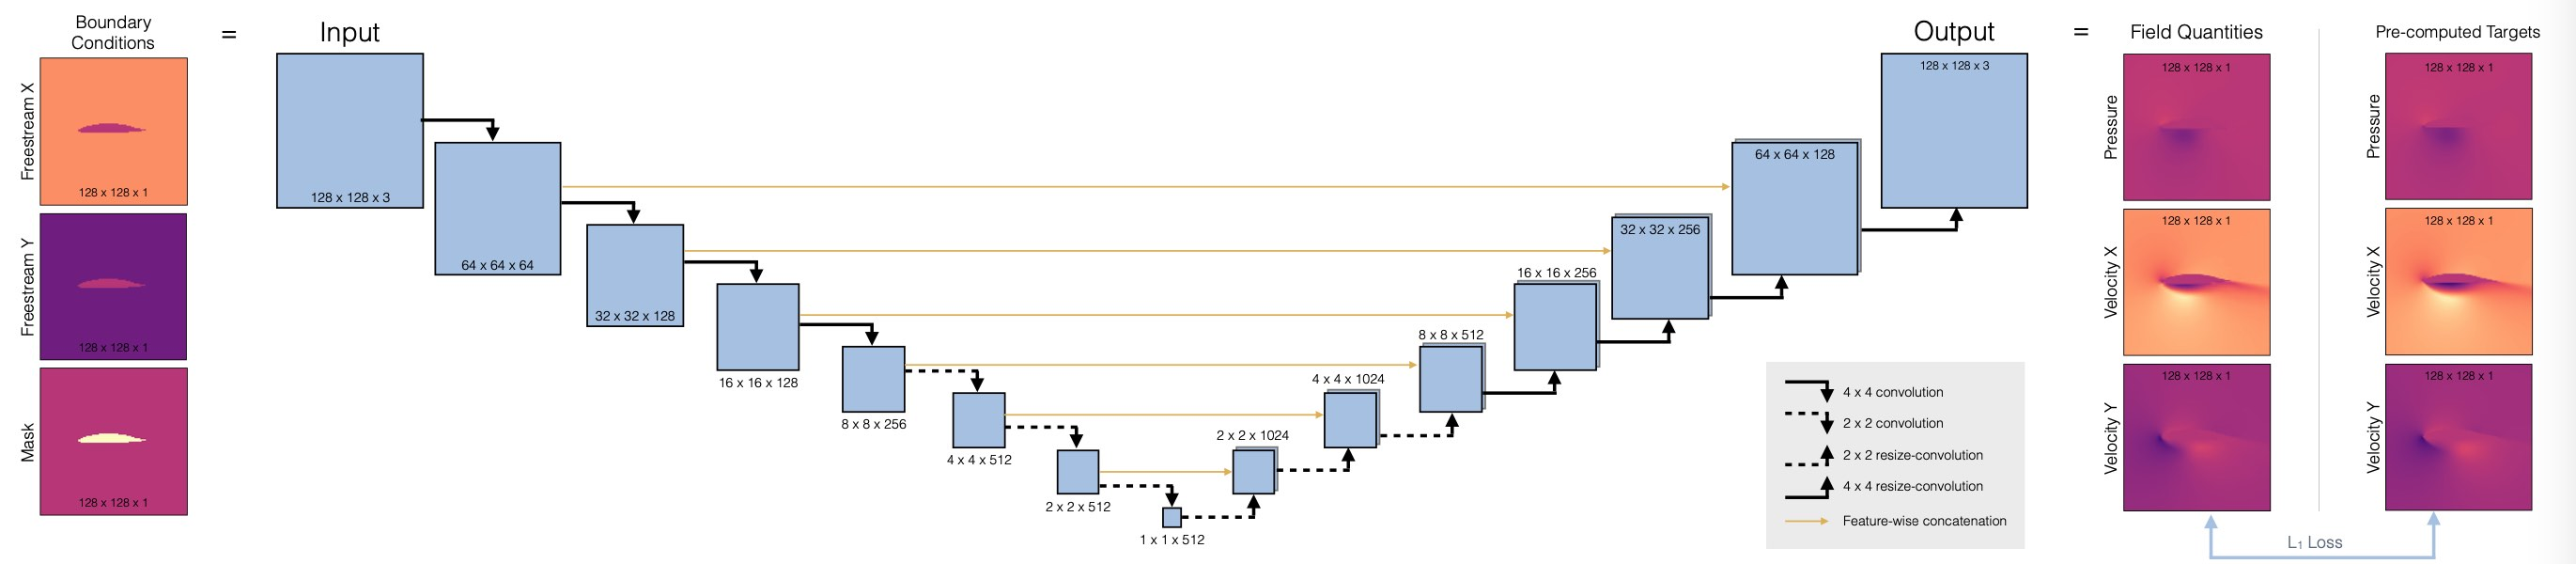
\includegraphics[width=1\linewidth]{images/pbdl_unet}
	\caption[pbdlunet]{Data driven U-Net from \cite{pbdl_book} learning an airfoil problem.}
	\label{fig:pbdlunet}
\end{figure}

\subsubsection{Neural Operators: Fourier Neural Operator}
Recall that an operator takes one function and gives another.  The purpose of neural operators is to extend spatially aware neural networks from finite-dimension to infinite dimension.  Like the functions above can have arbitrary resolution in parameter space $u(x) = y$, the same property is desired for neural network that can take and map an arbitrary temporal-spatial arrangement of states and parameters, as a function, at arbitrary resolution.  \cite{neural_operators} formally describes neural operators as well as provide proof of their universal approximation.  Formally, the purpose of neural operators is to learn a map between infinite dimensional spaces.  More intuitively, the purpose of neural operators is to learn a mapping between spaces of infinite resolution, from samples of finite resolution.
\begin{equation}
\mathcal{G}_\theta: \mathcal{A} \rightarrow \mathcal{U}
\end{equation}
Where $\theta \in R^p$ of finite dimension and $\mathcal{G}^\dagger$ is the actual map.  Neural operators can be trained to minimize the empirical risk:
\begin{equation}
\min_{\theta \in R^p} \frac{1}{n}\sum_{j=0}^{N-1}||u_j - \mathcal{G}(a_j)||^2_u
\end{equation}
Where $ a_j \sim u$ are independent and identically distributed samples so that $u_j = \mathcal{G}(a_j) + \mathcal{N}$.  

While $a_j$ and $u_j$ are treated as functions, they need to be sampled for computations.  If $D_j$ is the $n_j$ point discretization then $a_j|D_j,u_j|D_j \in R^{n_j}$ will be the collection of input output pairs. In practice, image planes are discretized to their resolution.  Important to the neural operator approach is that it is independent of the discretization \cite{neural_operators}.  In other words a model can be trained on multiple resolutions and infer on arbitrary resolutions.

The framework of a neural operator includes 3 steps \cite{neural_operators}:  

1. Lifting: A pointwise function lifts the input into a higher dimensional space $R^{d_a} \rightarrow R^{d_{v_0}},$ where typically $d_{v_0} > d_a$.  For images this is a 1x1 convolutional layer.  Recall that convolutions have depth across the input channels (parameters).

2. Iterative Kernel Integration:  Each hidden representation is mapped to the next $(v_t : D_t \rightarrow R^{d_{v_t}}) \rightarrow (v_{t+1} : D_{t+1} \rightarrow R^{d_{v_{t+1}}})$ by the sum of local linear operators, non-local integral operator, and bias function. 

3. Projection.  The last layer projects down to discrete space $R^{d_{v_T}} \rightarrow R^{d_u},$ where typically $d_{v_T} > d_u$ in a reflection of the first step.
\begin{figure}
	\centering
	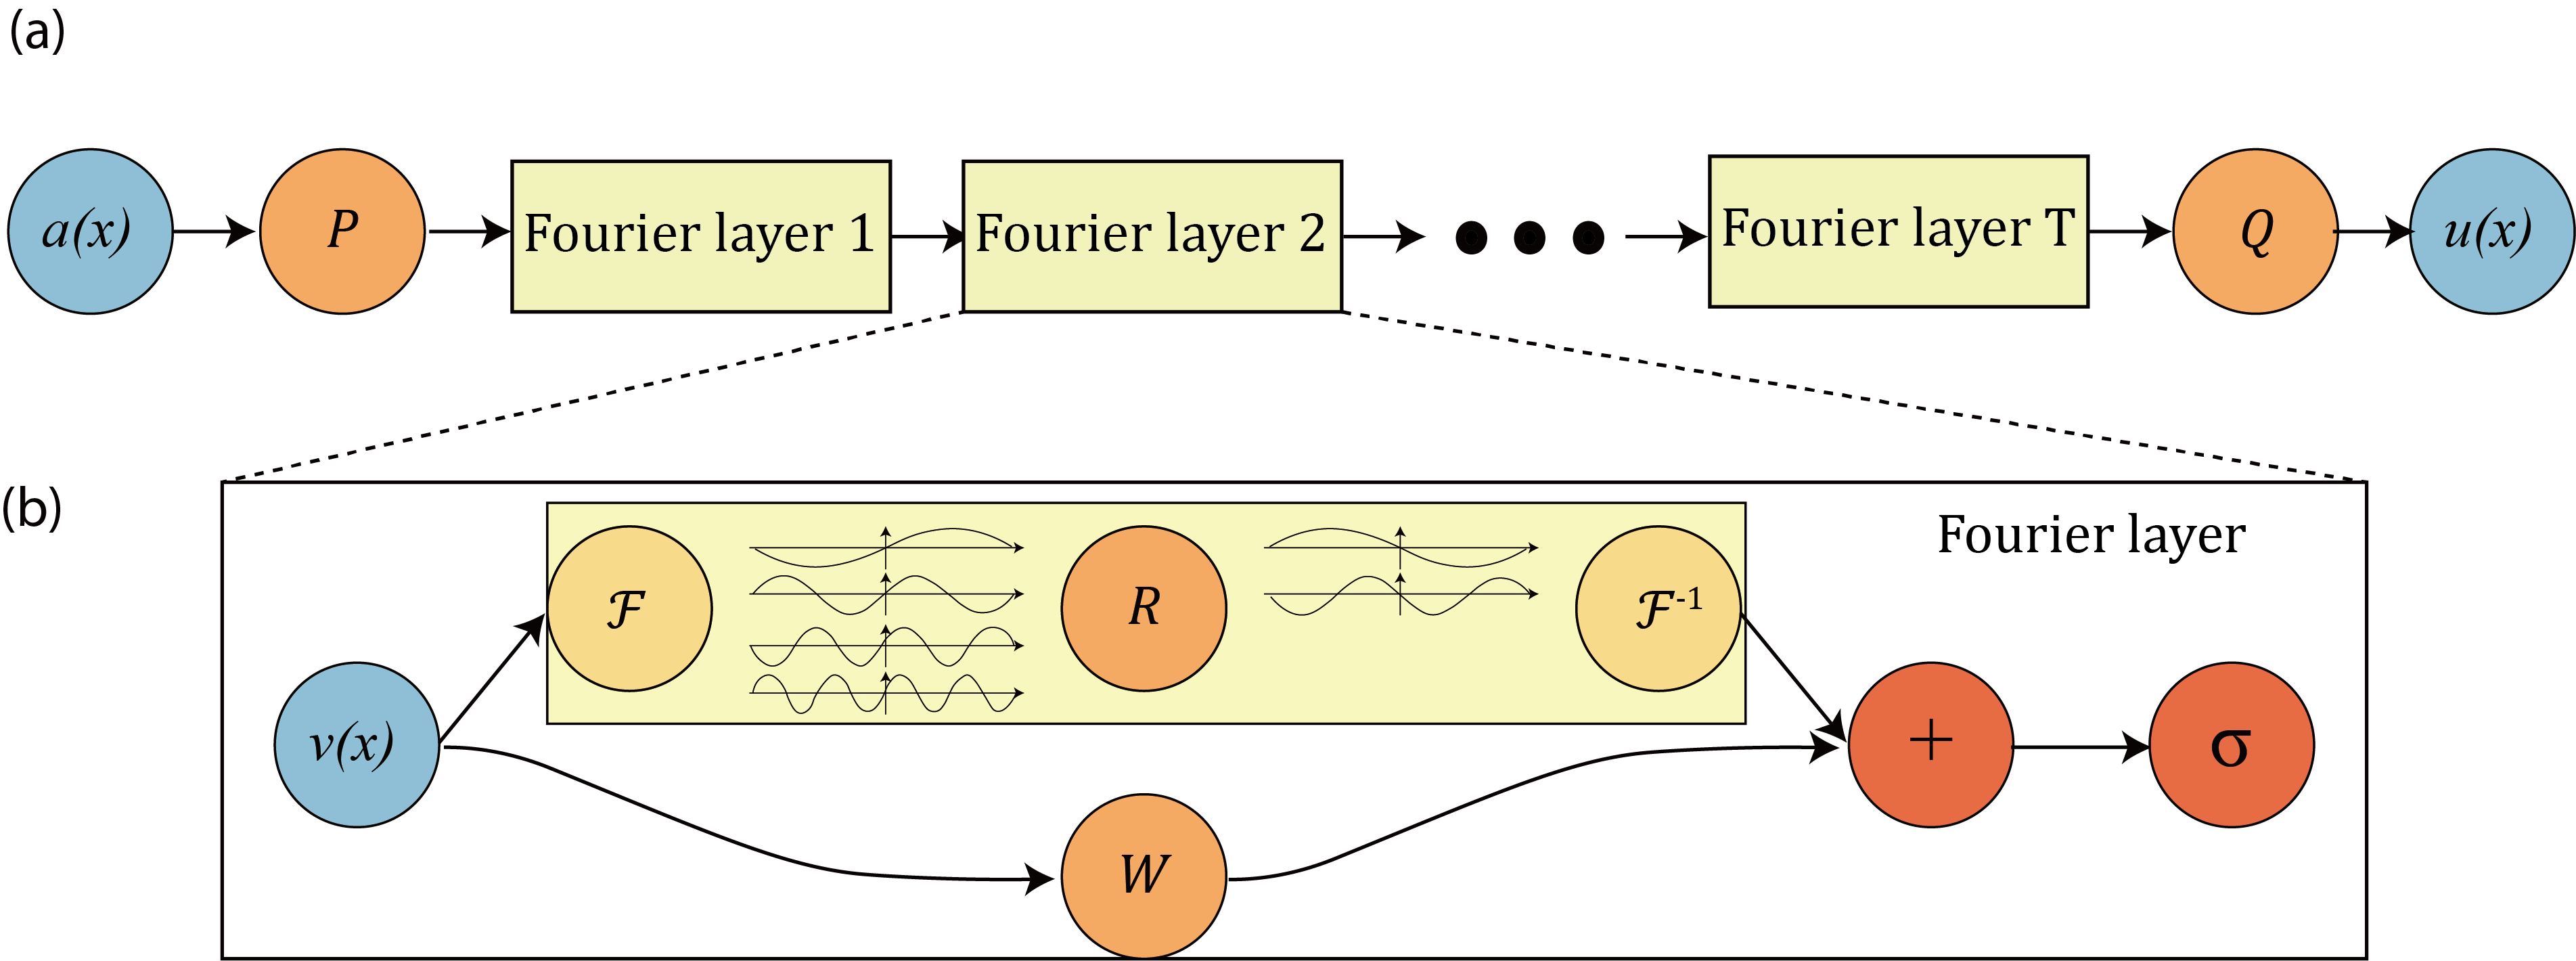
\includegraphics[width=1.0\linewidth]{images/FNO}
	\caption[FNO]{Full architecture of an FNO from \cite{fno}.  Step 1.) Lift $a(x) \rightarrow P$, for example with a 1x1 convolutional layer with stacks of 2D input parameters and states. Step 2.) Apply layers of integral operators and activation functions. Step 3.) Project back down to discrete samples  $Q(x) \rightarrow u(x)$, where $Q(x)$ is a neural network.  The Fourier layers copy the input $v(x)$ in two branches.  Top branch applies the Fouier transform $\mathcal{F}$, follow by a linear transform on the lower modes (filtering out the higher modes), and completed by an inverse Fourier transfer $\mathcal{F}^{-1}$. The bottom branch applies a local linear transform $\mathcal{W}$.}
	\label{fig:fno}
\end{figure}
The neural operator is an iterative architecture with a sequence of functions, operating on input after it is lifted into higher dimensions by a neural network $P(a(x))$.  Then several iterations of updates $v_t \rightarrow v_{t+1}$.  \cite{fno} defines this as:
\begin{equation}
v_{t+1}(x) := \sigma(\mathcal{W}v_t(x) + (\mathcal{K}(a;\phi)v_t)(x)), \forall x \in D 
\end{equation}
Which is the same as Figure \ref{fig:fno}.  Where the general kernel operator $\mathcal{K}$ is defined as:
\begin{equation}
(\mathcal{K}(a;\phi)v_t)(x) = \int_{D} \mathcal{K}(x, y, a(x), a(y); \phi)v_t(y)dy, \forall x \in D
\end{equation}
For FNOs in particular, the Fourier Integral Operator is defined by \cite{fno} as:
\begin{equation}
(\mathcal{K}(a;\phi)v_t)(x) = \mathcal{F}^{-1}(R_{\phi}\cdot (F_{v_t})(x), \forall x \in D
\end{equation}
Where $\phi$ are learnable parameters.  Which matches the architecture in figure \ref{fig:fno}.  Thus a full description of the network can be written as it is in \cite{nvidia_modulus}:
\begin{equation}
u_{net}(\Phi;\theta) = \mathcal{Q}\circ \sigma(W_{L} + \mathcal{K}_{L}) \circ ... \circ \sigma(W_{1} + \mathcal{K}_{1})\circ \mathcal{P}(\Phi), \quad \Phi=\left\{v_t(x); \forall x \in D\right\}
\end{equation}

Let's look at another example from Nvidia Modulus \cite{nvidia_modulus}, solving Darcy Flow with Fourier Neural Operator.  The Darcy PDE is:
\begin{equation}
-\nabla \cdot \left(k(\textbf{x})\nabla u(\textbf{x})\right) = f(\textbf{x}), \quad \textbf{x} \in D,
\end{equation}
Where $u(\textbf{x})$ is the flow pressure, $k(\textbf{x})$ is the permiability, and $f(\cdot)$ is the forcing function.  The boundary equation $u(\textbf{x}), \textbf{x} \in \partial D$ will be used for this example.   $\textbf{U}$ and $\textbf{K}$ will be discretized as 2D matrices (images essentially).  The problem develops a map between the permeability field and the pressure field $\textbf{K} \rightarrow \textbf{U}$.
\begin{figure}
	\centering
	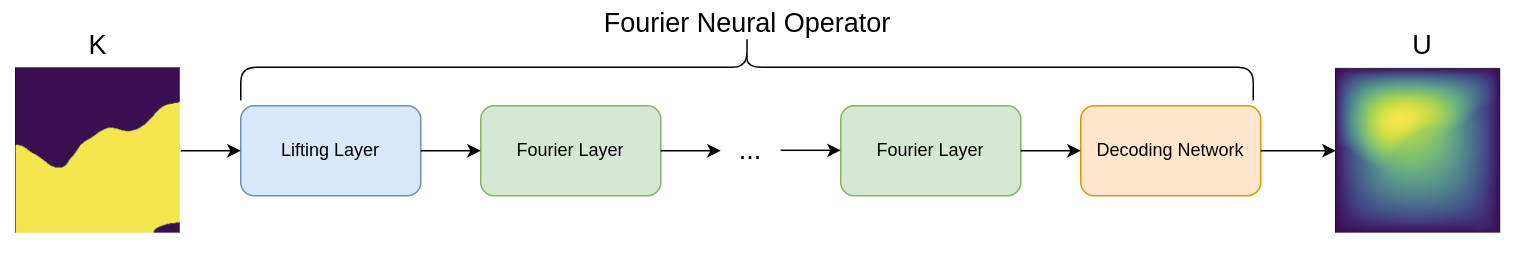
\includegraphics[width=1.0\linewidth]{images/fno_darcy}
	\caption[fno_darcy]{2D Darcy flow with Fourier Neural Operator from \cite{nvidia_modulus}. }
	\label{fig:fnodarcy}
\end{figure}
This particular problem was solved with a 2D FNO with 4 Fourier convolution layer with 32 features each.  There are no boundary conditions for this data-driven problem.  However the supervised training condition can be treated as a constraint.  The model is able to predict pressure fields for permeability fields it has not seen previously.
 
Neural operators are able to learn physical relationships generally, with arbitrary space parameterizations.  This makes them far more generally applicable than PINNs.  They are able to produce results for geometry or fields not in their training set.

\subsubsection{Neural Operators: Adaptive Fourier Neural Operator}
[NEED TO WRITE]

\subsection{Physics-Informed Neural Networks}
Physics-Informed Neural Networks include a conservation equation, in the form of a PDE, in their loss function.  When the conservation term is zero, there is zero error contributed by that part of the error term.
\begin{equation}
\textbf{L}_n = \frac{1}{J_L} \sum_{j=0}^{J_L -1} (\hat{u}_{n,j} - u_{n,j})^2 + \frac{1}{J_f}\sum_{j=0}^{J_f - 1}(f())^2
\end{equation}
$f() = 0$ when the physical quantity of concern is conserved.  PINNs take advantage of automatic differentiation to compute the necessary partial derivatives.  Two passed through the network are required for second derivatives.  Taking the Burger's equation example with Dirichlet boundary conditions from \cite{pinn_part1}:
\begin{gather}
u_t + uu_x - \frac{0.01}{\pi}u_{xx} = 0, x \in[-1, 1], t\in[0,1],\\
u(0,x) = -\sin(\pi x), \\
u(t, -1) = u(t, 1) = 0
\end{gather}
Then f(t,x) can be defined as:
\begin{equation}
f:= u_t + uu_x - \frac{0.01}{\pi}u_{xx}
\end{equation}
There are several ways to include boundary equations, including as part of the loss equation such as in Figures [\ref{fig:ppinn-schematic}] and [\ref{fig:xtfcscheme}].  In Nvidia Modulus \cite{nvidia_modulus} boundary conditions and initial conditions can be implemented as data constraints (i.e. as labels for a given u(x,t)) and loss for them is handled in a similar manner to data loss. 
\begin{figure}
\centering
	\begin{subfigure}{0.49\textwidth}
		\centering
		\includegraphics[width=1\linewidth]{"images/ppinn schematic"}
		\caption[ppinn]{Diagram of PINN from \cite{ppinn}.}
		\label{fig:ppinn-schematic}
	\end{subfigure}
	\begin{subfigure}{0.49\textwidth}
		\centering
		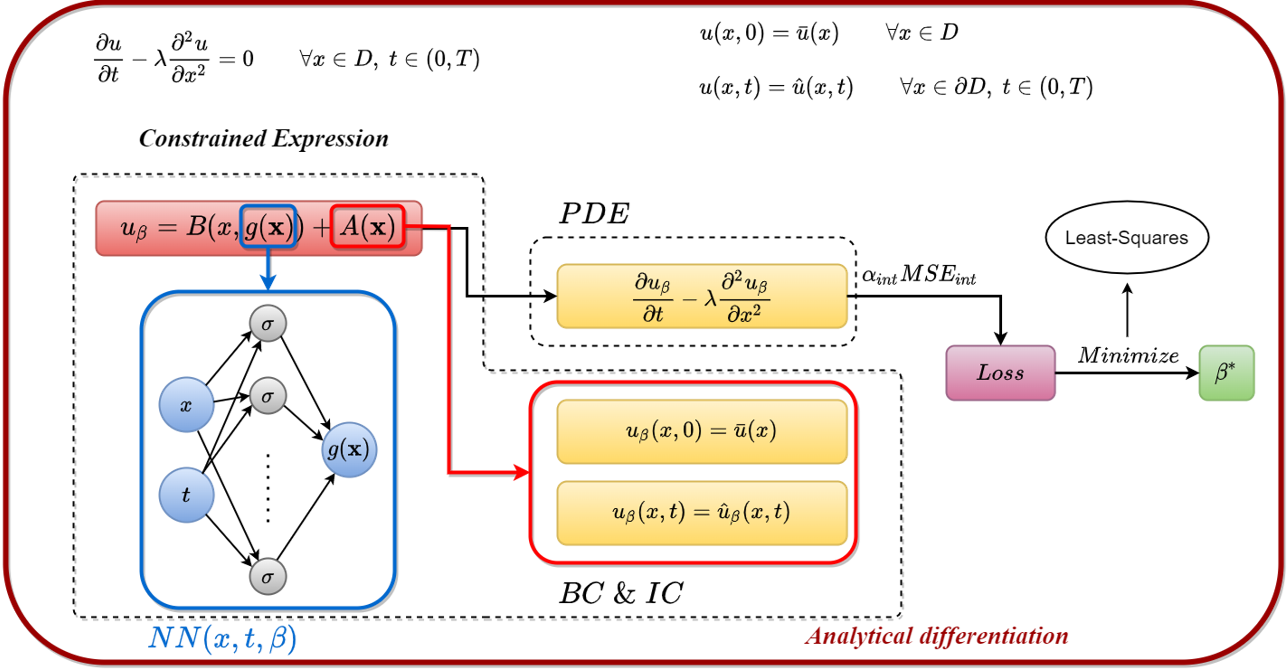
\includegraphics[width=1\linewidth]{images/Xtfc_scheme}
		\caption[pinnwiki]{Xtfc of PINN schematic from wikipedia.}
		\label{fig:xtfcscheme}
	\end{subfigure}
\end{figure}

Let's look at a simple example in Nvidia's Modulus, the lid driven cavity \cite{nvidia_modulus}.  In this example, incompressible fluid is in a container whose lid moves in the +x direction and the other walls do not move.  For this problem, continuity and momentum equations are needed:
\begin{gather}
\frac{\partial u}{\partial x} + \frac{\partial v}{\partial y} = 0 \\
u\frac{\partial u}{\partial x} + v\frac{\partial u}{\partial y} + \frac{\partial p}{\partial x} - \textit{V}(\frac{\partial^2u}{\partial x^2} + \frac{\partial^2u}{\partial y^2})= 0 \\
u\frac{\partial v}{\partial x} + v\frac{\partial v}{\partial y} + \frac{\partial p}{\partial x} - \textit{V}(\frac{\partial^2v}{\partial x^2} + \frac{\partial^2v}{\partial y^2})= 0
\end{gather}
Which creates the constraints:
\begin{equation}
\textbf{L} = \frac{V}{N}\sum_{n = 0}^{N - 1}((0 - continuity(x_n, y_n))^2 + (0 - momentum_x(x_n, y_n))^2 + (0 - momentum_y(x_n, y_n))^2) 
\end{equation}
Initial conditions and boundary conditions are implemented in Modulus as data contraints, sampled from the problem domain.  The interior of the container is constrained to the PDEs.  Samples from the top wall have output labels of $u=1.0, v = 0.0$.  The samples from the other walls have labels $u=0.0, v = 0.0$.  In order to help the neural network learn boundary constraints, the engineer can determine how many samples should come from the boundary and how many should come from the interior.  The corner between the top wall and the side walls causes a discontinuity.  To help the neural network learn faster, modulus can take a lambda weighting for the boundary conditions.  In this case the top wall is modified with $\lambda = (u = 1.0 - 20.0|x|, 1.0)$.  This is visualized in Figure \ref{fig:ldclambda}.
\begin{figure}
	\centering
	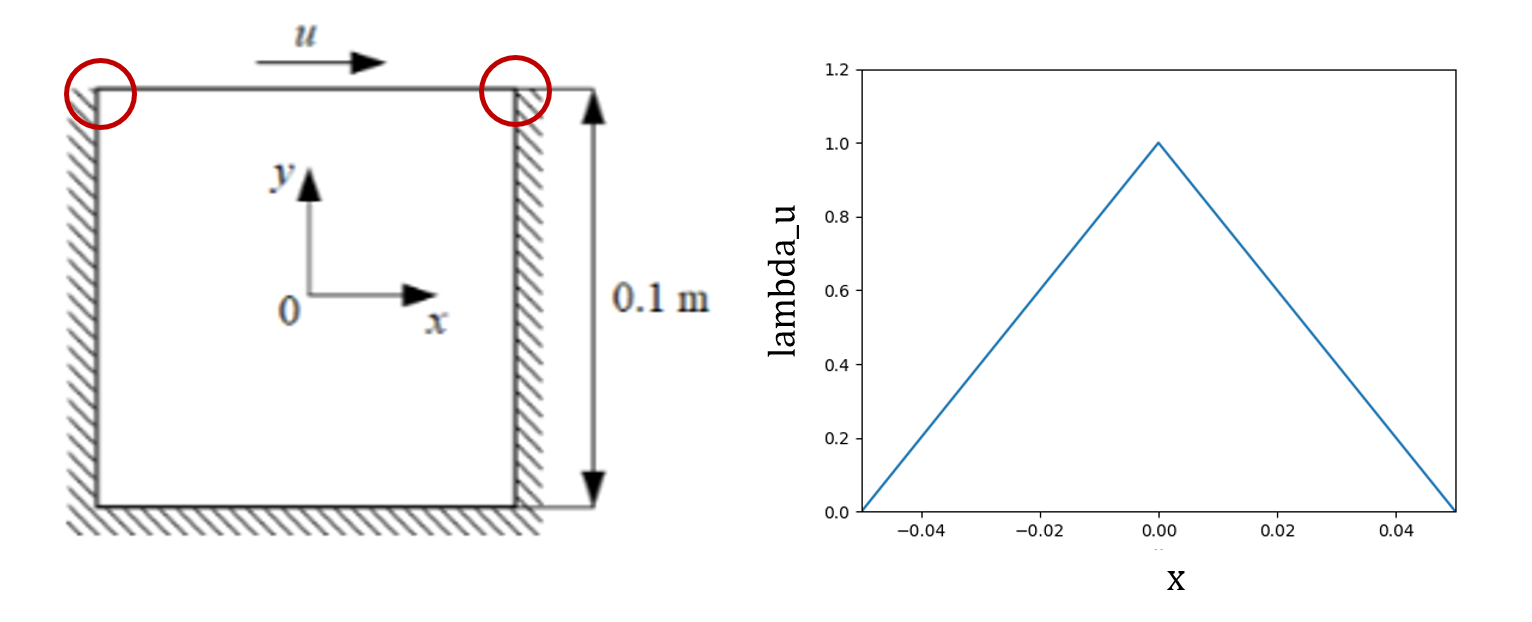
\includegraphics[width=1\linewidth]{images/ldc_lambda}
	\caption[ldc_weighting]{Visualization of lambda weighting for the top wall boundary constraint in the lid driven cavity example from \cite{nvidia_modulus}.}
	\label{fig:ldclambda}
\end{figure}

The model trains fairly quickly on a relatively old computer (when making concessions due to limited memory).  The tensorboard in Figure \ref{fig:screenshot-2022-05-09-at-17-19-07-tensorboard} shows the results.  If you have the compute and memory resources you can compare results to the CFD software package OpenFOAM.
\begin{figure}
	\centering
	\includegraphics[width=0.7\linewidth]{"images/Screenshot 2022-05-09 at 17-19-07 TensorBoard"}
	\caption[ldc_results]{Results from training a neural network on the lid driven cavity example from Modulus.}
	\label{fig:screenshot-2022-05-09-at-17-19-07-tensorboard}
\end{figure}

The most obvious use case of PINNs is to learn a sparsely sampled problem.  We can consider a sparsely sampled problem as one where the order of magnitude of the number of observations is less than the order of magnitude of the number of parameters.  In such a case, including PDE based losses may augment the data and help the network learn the problem.  An important advantage of PINNs over traditional solvers is the ability to solve them over parameterized geometries.  \cite{neural_operators} notes that PINNs are only useful for learning a single problem.  Any spatial dependencies are encoded into the network.

\subsubsection{Neural Operators: Physics-Informed Neural Operator}
[NEED TO WRITE]

\subsection{Transfer Learning from Simulations}
Transfer learning involves re-purposing a neural network, trained on one task for another.  This can involve replacing and training the final few layers of a neural network or retraining the whole thing.  In the case that a high fidelity physical simulation exists, a surrogate would first be trained to approximate the simulation.  Then the surrogate can be further trained on real data.  

As an example, we have a signal power loss application.  In order to enable transfer learning, we had to implement the state-of-the-art numerical approximation.  We enabled parallel evaluation with CUDA, in order to enable large data generation quickly.  We implement the functions as described in \cite{Nicole_SigProp}:
\begin{equation}
Loss = f(\textbf{h}_0, \textbf{h}_1, \textbf{h}_2, \textbf{d}_1, \textbf{d}_2, \textbf{freq})
\end{equation}
Where the inputs are all vectors to enable parallel computation of many examples.  Every entry $i$ is an example.
\begin{equation}
Loss_i = FSPL_i + LOS_i + NLOS_i
\end{equation}
Where FSPL is the loss that occurs in the Fresnel Zone, LOS is the loss that occurs when the Freznel Zone is obstructed but the line-of-sight remains unobstructed, and NLOS is the loss that occurs when the line-of-sight is obstructed.  The losses are defined as:
\begin{equation*}
	FSPL_i =\begin{cases}
		20\log(d_{1,i} + d_{2,i}) + 20\log(f_{GHz}) + 92.45dB \quad &\text{if} \, v\le-1.0 \\
		0 \quad &\text{if} \, otherwise \\
	\end{cases}
\end{equation*}
\begin{equation*}
	LOS_i =\begin{cases}
		6.0(1.0 - \frac{C_{obs}}{R_{FR}})dB \quad &\text{if} \, 0.0 < v < 1.0 \\
		0 \quad &\text{if} \, otherwise \\
	\end{cases}
\end{equation*}
\begin{equation*}
	NLOS_i =\begin{cases}
		6.9 + 20\log(\sqrt{(v-0.1)^2 + 1.0} + v -0.1)dB \quad &\text{if} \, v \ge 0.0 \\
		0 \quad &\text{if} \, otherwise \\
	\end{cases}
\end{equation*}
Where,
\begin{gather}
R_{FR,i} = 0.6(547.533\sqrt{\frac{d_{1,i}d_{2,i}}{f_{MHz}(d_{1,i} + d_{2,i})}})\\
C_{obs,i} = h_i = h_{0,i} + h_{ER,i} - h_{1,i} - \frac{(h_{2,1} - h_{1,i})}{(d_{1,i} + d_{2,i})}d_{1,i}\\
v_i = h_i\sqrt{\frac{2(d_{1,i} + d_{2,i})}{\lambda d_{1,i}d_{2,i}}}\\
h_{ER,i} = \frac{d_{1,i}d_{2,i}}{16.944}\\
\lambda = \frac{299792458}{freq_{Hz}}
\end{gather}
\begin{figure}
	\centering
	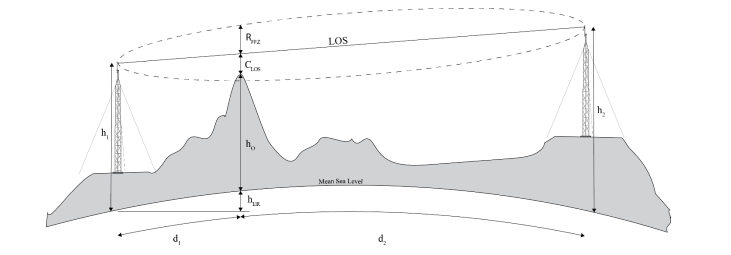
\includegraphics[width=1.0\linewidth]{images/SignalLoss}
	\caption[SigProp]{Signal Loss graphic from \cite{Nicole_SigProp}.}
	\label{fig:signalloss}
\end{figure}

We can use this simulation to train a neural network to approximate it's results.  We can then use transfer learning on a limited dataset.  Such a training methodology makes use of prior physical knowledge and available data.

\subsection{Validation with High Fidelity Simulations}
Another way to take advantage of high fidelity simulations is to use them as part of validation.  This technique can effectively use the limited, expensive data from these simulations as part of hyper-parameter tuning.  This induces a bias in the surrogate model towards the results of the simulation.
\subsection{Neural Adapter}
A neural adapter, as described by \cite{zubov2021neuralpde} is similar to transfer learning.  Instead of retraining a neural network or adding layers to it, a new neural network is trained to adapt a previously trained model to the new problem domain.  Figure \ref{fig:neuraladapter} shows the general architecture of the problem.  
\begin{figure}
	\centering
	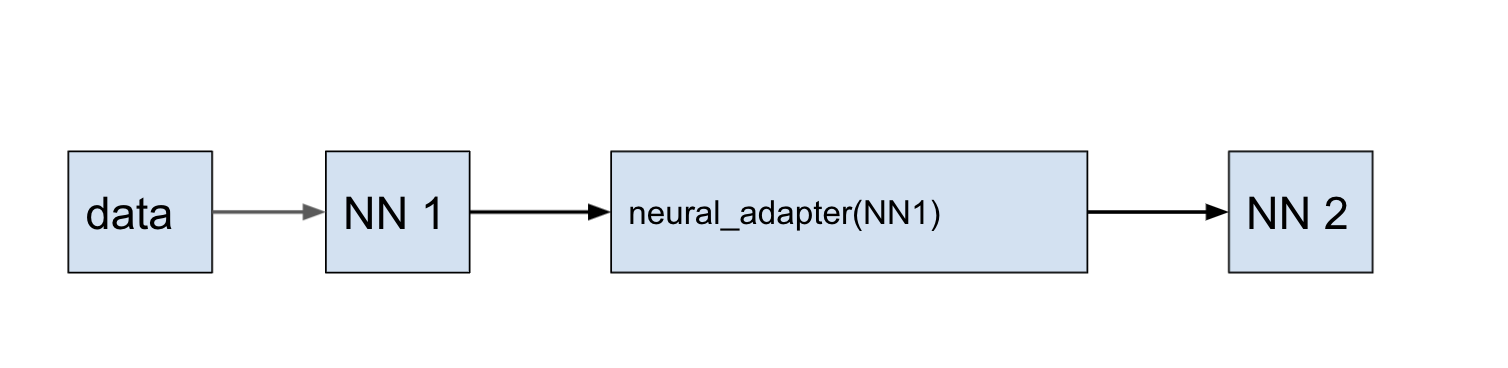
\includegraphics[width=1.0\linewidth]{images/neural_adapter}
	\caption[neural adapter]{Neural adapter architecture by \cite{zubov2021neuralpde}}.
	\label{fig:neuraladapter}
\end{figure}
Not only could this be done with neural networks, but the results from other models could be corrected by a neural network to better fit the problem domain.  The results of existing physical models could be adjusted to better fit real data.  The problem would be of the form:
\begin{equation}
arg min_\theta \frac{1}{2}\sum_{k=0}^{K_L - 1}(N(S(\textbf{x}_k), \boldsymbol{\theta}) - \hat{\textbf{y}}_k)^2
\end{equation}
Where $S(\textbf{x}_k)$ is the output from the simulation.
\subsection{Differentiable Simulations}
[NEED TO WRITE]
\subsection{Inverse Problems}
[NEED TO WRITE]
\subsection{Implicit Model Representations}
Because we are researching surrogate models for EOIR and light transport, we will likely need to perform research into 3D model, texture, and lighting representations useful for learning problems.  This has been done with the output of neural networks controlling triangle meshes, voxels, and neural adaptors for lighting.  Recently, neural network representations have been used to reconstruct 3D scenes.  These representations are implicit and can be evaluated at arbitrary resolution.
\subsubsection{Neural Radiance Fields}
[NEED TO WRITE]
\subsection{Uncertainty in Physics-Based Neural Networks}
There are uncertainties and possible errors in data, measurements, physics models, and surrogate models.  We would like some way for our models to couch the uncertainty of their inferences.  The uncertainty from data is called aleatoric uncertainty.  The uncertainty in our model is called epistemic uncertainty.  The book Physics Based Deep Learning [cite it] describes an approach using Bayesian Neural Networks (BNNs) to make posterior inference possible.  The goal of posterior inference is to reproduce the full output distributions.  BNNs do this by assuming probability distributions for the parameters.  At this point it is still very difficult to train BNNs.

One of the major advantages of fast surrogate models is the ability to perform Monte Carlo simulations and get statistical distribution on the likely outcomes.  One of the major limitations of large physics simulations is that they either take a very long time to run or are uselessly coarse.  Because of this long run time, variational statistics (such that you might get from a Monte Carlo) cannot be calculated.  This is a famous issue with climate models, where each paper represents only one or a few model runs.  One of the purposes of Nvidia’s Earth-2 is to enable faster execution of weather and climate simulations.  This can then enable an ensemble of many simulations with varying model starting parameters.  After searching the parameter space, we can make statements on the relative likelihood of certain system states. 

\section{Packages}
Physics-based neural networks can be implemented fairly easily in any neural network framework, as \cite{pbdl_book} does with PyTorch.  In fact, since none of the core techniques are black boxes, any of these methods could be re-implemented in a fast language if necessary.  However, there are some packages available that make quick development of physics-based neural networks easier. 

1.) Nvidia Modulus, \cite{nvidia_modulus} is easy to use, well documented, and implements much of the latest research in physic-bases neural networks.  Works with PyTorch.

2.) NeuralPDE.jl, \cite{zubov2021neuralpde} is part of SciML.  And is a Julia language package with PINNs and deep Forward-Backwards Stochastic Differential Equations solvers. 

3.) SciAnn: Neural Networks for Scientific Computations, \cite{haghighat2021sciann}, a package using TensorFlow and Keras.

4.) DeepXDE, \cite{lu2021deepxde},  a library containing algorithms for PINNs and DeepONets.  Compatible with Tensorflow and PyTorch.

\section{Evaluation Metrics}
In addition to metrics such as accuracy and error, domain specific evaluation metrics should be adopted to fully assess the performance of surrogate models.  For example, Lai et al [cite Bridging by Lai et al 2019], compared several unsupervised loss functions for image reconstruction.  These methods went beyond simple cosine similarity or mean squared error, in order to encourage semantically similar reconstructions.  They also compared and qualified reconstructions produced by models trained by various loss functions to human preferences.  For our purposes, we may construct evaluation metrics and loss functions that focus on the most important aspects of the simulation results (ex: shape and contrast vs mean intensity and noise). 

\bibliographystyle{plain}
\bibliography{reference}

\end{document}





